\documentclass[11pt,a4paper]{ivoa} 
\input tthdefs

\usepackage{makecell}
\usepackage{listings}
\usepackage{adjustbox}
\usepackage[normalem]{ulem}
\usepackage{fancyvrb}
\usepackage{appendix}
\lstloadlanguages{C}
\lstset{flexiblecolumns=true,numberstyle=\small,showstringspaces=False,
  basicstyle=\ttfamily,defaultdialect=[latex]tex,language=tex}

\usepackage[colorinlistoftodos]{todonotes}

\usepackage[utf8]{inputenc}

\usepackage{titlesec}
\titleformat{\paragraph}
{\normalfont\normalsize\bfseries}{\theparagraph}{1em}{}
\titlespacing*{\paragraph}
{0pt}{3.25ex plus 1ex minus .2ex}{1.5ex plus .2ex}


\definecolor{texcolor}{rgb}{0.4,0.1,0.1}
\newcommand{\texword}[1]{\texttt{\color{texcolor} #1}}

\iftth
  \newcommand{\BibTeX}{BibTeX}
\fi
\newcommand\apj{The Astrophysical Journal}
\newcommand\jcap{Journal of Cosmology and Astroparticle Physics}
\newcommand\prd{Physical Review D}
\newcommand\aap{Astronomy \& Astrophysics }

\iftth
 \newcommand{\comicstuff}[1]{
    \begin{html}<span class="comic">#1</span>\end{html}}
\else
  \newcommand{\comicstuff}[1]{(HTML exclusive material)}
\fi
\customcss{custom.css}

\newcommand\ada[1]{\textcolor{red}{\textbf{#1}}}
\newcommand\daniel[1]{\textcolor{blue}{\textbf{#1}}}  
\newcommand\pierre[1]{\textcolor{orange}{\textbf{#1}}} 

\title{MOC: Multi-Order Coverage map}

\ivoagroup{Applications}

\author{Pierre Fernique (CDS)}
\author{Ada Nebot (CDS)}
\author{Daniel Durand (CADC)}
\author{Matthieu Baumann (CDS)}
\author{Thomas Boch (CDS)}
\author{Giuseppe Greco (EGO-Virgo)}
\author{Tom Donaldson (STScI/NASA)}
\author{Francois-Xavier Pineau (CDS)}
\author{Mark Taylor (University of Bristol)}
\author{Wil O'Mullane (Vera C. Rubin Observatory)}
\author{Martin Reinecke (Max Planck)}
\author{S\'{e}bastien Derri\`{e}re (CDS)}

\editor{Pierre Fernique}
\editor{Ada Nebot}
\editor{Daniel Durand}


\previousversion[http://ivoa.net/documents/MOC/20191007]{Version1.1}
\previousversion[http://ivoa.net/documents/MOC/20140602]{Version1.0}

\begin{document}

\begin{abstract}
This document describes the Multi-Order Coverage map method (MOC)
version 2.0 to specify arbitrary coverages for sky regions and/or time
coverages and potentially other dimensions. The goal is to be able to
provide a very fast comparison mechanism between coverages. The
mechanism is based on a discretization of space and time
dimensions. The system is based on the definition of a specific storage
of the map coverage using predefined cells hierarchically grouped
which makes it easy to produce and use for exploring astronomical
collections. There are already a few applications and libraries which
are taking advantage of this major evolution of the MOC standard. 
\end{abstract}

\listoffigures
\listoftables  
%\todototoc
%\listoftodos[Issues which need attention]


\section*{Acknowledgments}
This work has been supported by the ESCAPE project (the European
Science Cluster of Astronomy \& Particle Physics ESFRI Research
Infrastructures) that has received funding from the European Union's
Horizon 2020 research and innovation Programme under the Grant
Agreement n.\ 824064.

\section*{Conformance-related definitions}
The words ``MUST'', ``SHALL'', ``SHOULD'', ``MAY'', ``RECOMMENDED'',
and ``OPTIONAL'' (in upper or lower case) used in this document are to
be interpreted as described in IETF standard RFC2119
\citep{std:RFC2119}.

The \emph{Virtual Observatory (VO)} is a general term for a collection
of federated resources that can be used to conduct astronomical
research, education, and outreach.  The
\href{http://www.ivoa.net}{International Virtual Observatory Alliance
  (IVOA)} is a global collaboration of separately funded projects to
develop standards and infrastructure that enable VO applications.

\begin{figure}[!htbp]
\begin{center}
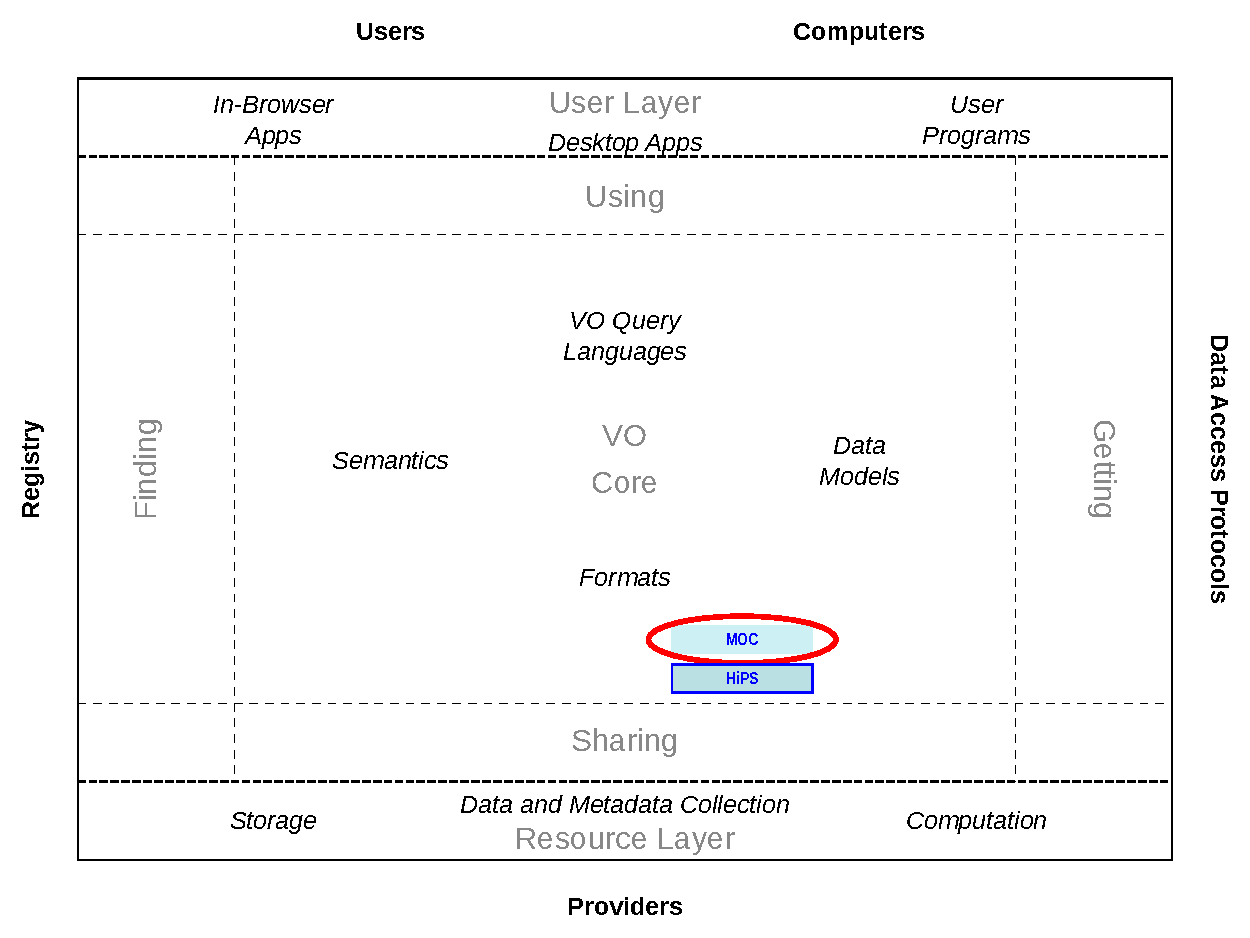
\includegraphics[width=0.9\textwidth]{role_diagram.pdf}
\end{center}
\caption[IVOA architecture diagram]{Architecture diagram for Multi-Order Coverage map.}
\label{fig:ivoadiagram}
\end{figure}

\section{Introduction}
This document is a major release of
the already existing encoding method recommendation \emph{Multi-Order
  Coverage} map \citep[MOC~1.1,][]{2019ivoa.spec.1007F}. We generalize the MOC
originally limited to space dimension (Space MOC, SMOC) to the time
dimension (Time MOC, TMOC), and space and time dimensions (Space-Time
MOC, STMOC). Figure~\ref{fig:ivoadiagram} illustrates the role MOC2.0
plays within the IVOA architecture \citep{2021ivoa.spec.1101D}.

The encoding method described in this document allows one to define
and manipulate space and time coverage in such a way that basic
operations like union, intersection, equality test can be performed
very efficiently. This methodology allows VO applications and
data servers to build efficient
procedures to perform such operations on observations and catalogs. 
In the next sections we will describe the different MOCs and their
encoding standards.

\section{The rationale}
\label{sec:usecases}
The goal behind the MOC is to get a method to manipulate coverages in
order to provide very fast union, intersection and
equality operations between them. In order to accomplish this task, we
based the system on a regular and hierarchical discretization as
exposed below. The standard MOC1.0 was limited to space, but for a
multitude of use cases in astronomy we need the notion of time to be
properly integrated, e.~g.:
\begin{itemize}
\item What are the space and time coverages of the 2MASS observations
  and are there any observations which are coincidental with the HST
  archive?
\item Which are the astronomical catalogs which have data for a list
  of Supernova events within a given time window?
\item Are there any other observations coincidental with this
  gravitational wave detection given its time and spatial coordinates?
\item Are there quasi-simultaneous observations (within a given time
  window) of these two surveys for a list of eclipsing binaries?
\item Find the intersection between the SDSS coverage and the
  ephemeris of this Near Earth Object, was it observed by SDSS? And
  by Galex? By both missions simultaneously? If so, are there
  detections within the source catalogues?
\item Has Neptune been observed by DSS?
\end{itemize}

It was possible to answer those questions with MOC1.0 standard and
other VO tools but the amount of manipulation and computation was
quite a big hurdle for the researchers. With MOC2.0 it is possible
to answer these questions in a few milli-seconds. Another example
of usage would be the visual inspection of the spatio-temporal
coverage of PanSTARRS observations (see Figure~\ref{fig:panstarrs}). 
The choice of a temporal resolution and a spatial resolution makes it
possible to obtain a MOC of a desired data volume. 

\begin{figure}[!ht]
\begin{center}
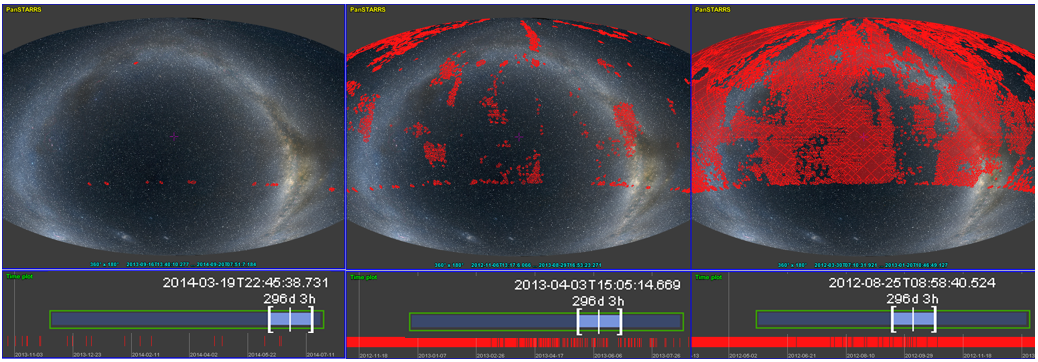
\includegraphics[width=\textwidth]{panstarrs.png}
\caption{PanSTARRS observations and the associated spatial and
  temporal coverage within three different periods of time.
  The volume of the PanSTARRS MOC at a temporal resolution
  of about 17 minutes and spatial resolution of 52 arcsec is 320\,MB.}
\label{fig:panstarrs}
\end{center}
\end{figure}

\subsection{Comparing the coverage of multiple data sets}
The computation of data set intersections using the MOCs is simple (it
is simply a list comparison). The result of any operation is itself a
MOC which can be used in further operations. For instance it is
possible to compute the intersection of Saturn's ephemeris and
the spatio-temporal coverage of HST ACS observations, and subsequently,
query a database for retrieving images for which time and position
fall within this intersection (see Fig.~\ref{fig:stmoc-saturn}). 

\begin{adjustbox}{center,caption={Intersection of HST ACS observations
      and Saturn ephemeris Space-Time-MOC},label={fig:stmoc-saturn},
    nofloat=figure,vspace=\bigskipamount}
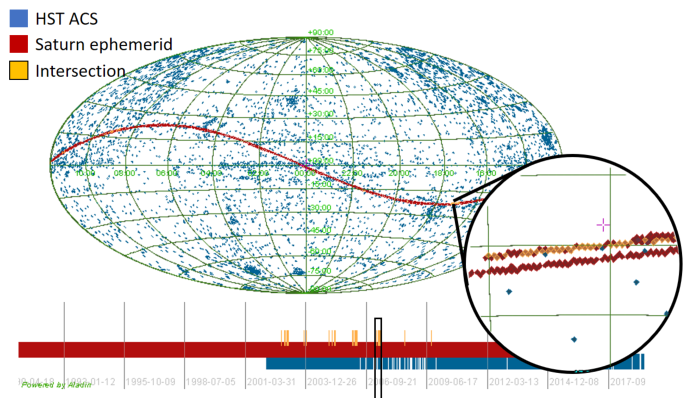
\includegraphics[width=\textwidth]{stmoc_op.png}
\end{adjustbox}

\subsection{Query databases using MOC}
In principle, querying a positional database using complex sky region
coverage is possible using ADQL. However, this is rarely possible
when the sky region has to be described as unions and intersections of
sub-regions to cover a complex, non regular area. In practice, most
existing ADQL implementations only support simple regions
(cones, boxes, polygons), and can rarely deal with unions and
intersections unless by joining independent queries – and this even if
the described region is, in fact, empty!  If databases are adapted to
supporting MOC based queries, they will offer then a useful method
allowing any kind of sky region query. In addition, if the internal
spatial index of the database is itself based on HEALPix, the
filtering will then be straightforward and all the intermediate sky
computations will be removed providing an optimal response time.

\subsection{Gravitational Wave localisations}
The contours of a gravitational-wave sky localization are constructed
as follows. The pixels from most probable to least are ranked, and summed
up to get a fixed level of probability \citep{2014ApJ...795..105S}.
In practice, the HEALPix pixels inside a given contour plot are extracted,
and the MOC coverage is generated from the table made up from the pixels.
Every single level of probability can be used as a regular MOC even in the case in
which the sky localization is irregularly shaped with disjoint regions.
This coding technique allows for an extra fast integration in the existing
Virtual Observatory structures and tools\footnote{\url{https://emfollow.docs.ligo.org/userguide/}}. 
The 2D contours of a GW sky localization can be visualised and
manipulated using Aladin Desktop, allowing one to compare them with
existing surveys, overlap sky map generations with increasing accuracy
and computational cost and query the VizieR database. 
These sets of tasks can also be performed via Python using the astropy
affiliated package mocpy\footnote{\url{https://cds-astro.github.io/mocpy/}},
efficiently displayed in javascript applications
with Aladin Lite, and integrated within Jupyter notebooks through the
ipyaladin widget\footnote{\url{https://pos.sissa.it/357/031/pdf}}. 

Adding temporal information in a space MOC encoding can provide a
systematic approach in extracting information from follow-up campaigns
involving tens of ground and space-based observatories in searching
for gravitational-wave counterparts.
For illustrative purposes only, a potential use of the time-space MOC
is provided when a kilo/macronova emission is a credible counterpart of a
gravitational-wave event. 
Figure~\ref{fig:gw} shows a mock electromagnetic
follow-up campaign of a gravitational-wave sky localization over a period
of time (left panel), a schematic kilonova light-curve and
temporal coverage of observations (top right panel) and associated
spatial coverage (bottom right panel). This approach permits us to depict
the approximate timeline of the instruments involved in the observational
campaign and place constraints on the emission properties during the
source evolution.

\begin{figure}[!htbp]
\begin{center}
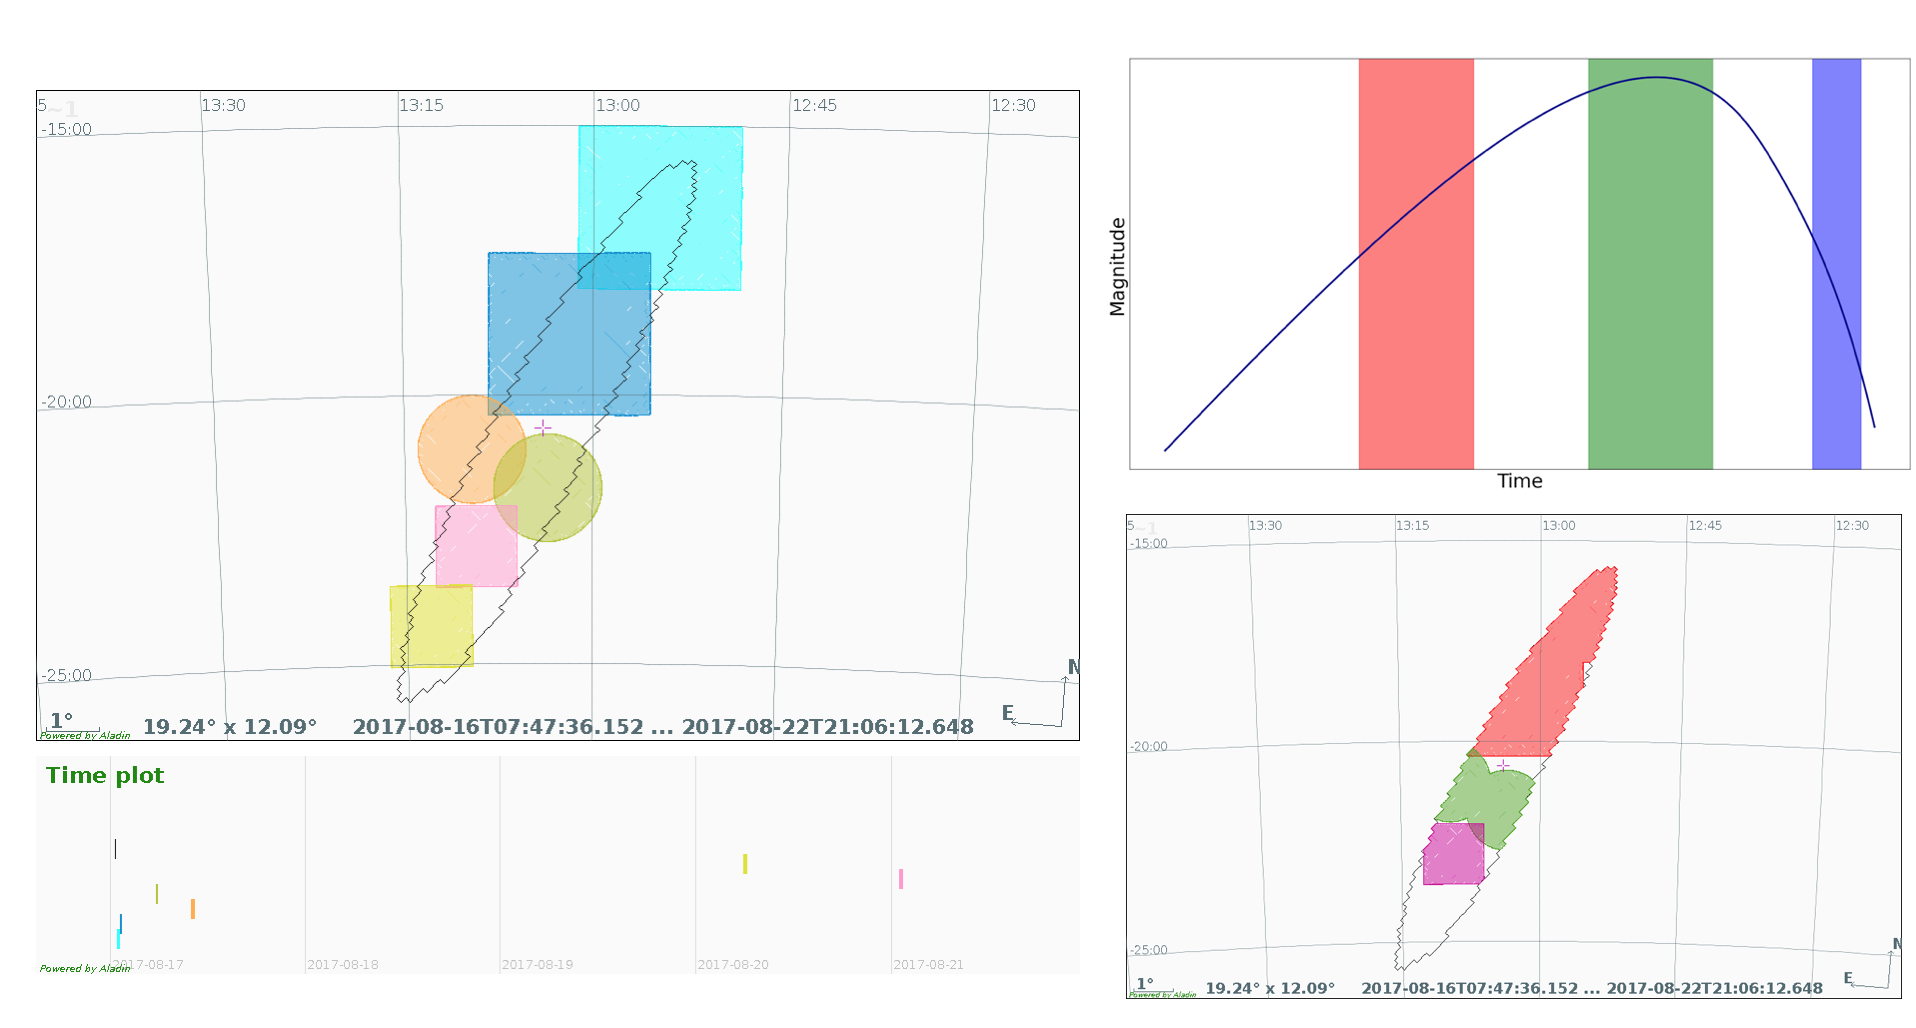
\includegraphics[width=\textwidth]{kilo.png}
\end{center}
\caption{A mock electromagnetic follow-up campaign
  of a gravitational-wave sky localization over a time period (left).
  A schematic kilonova light-curve with the observations temporal
  coverage (top right) and associated spatial coverage (bottom right).}
\label{fig:gw} 
\end{figure} 

%\begin{figure}[!htbp]
%\begin{center}
%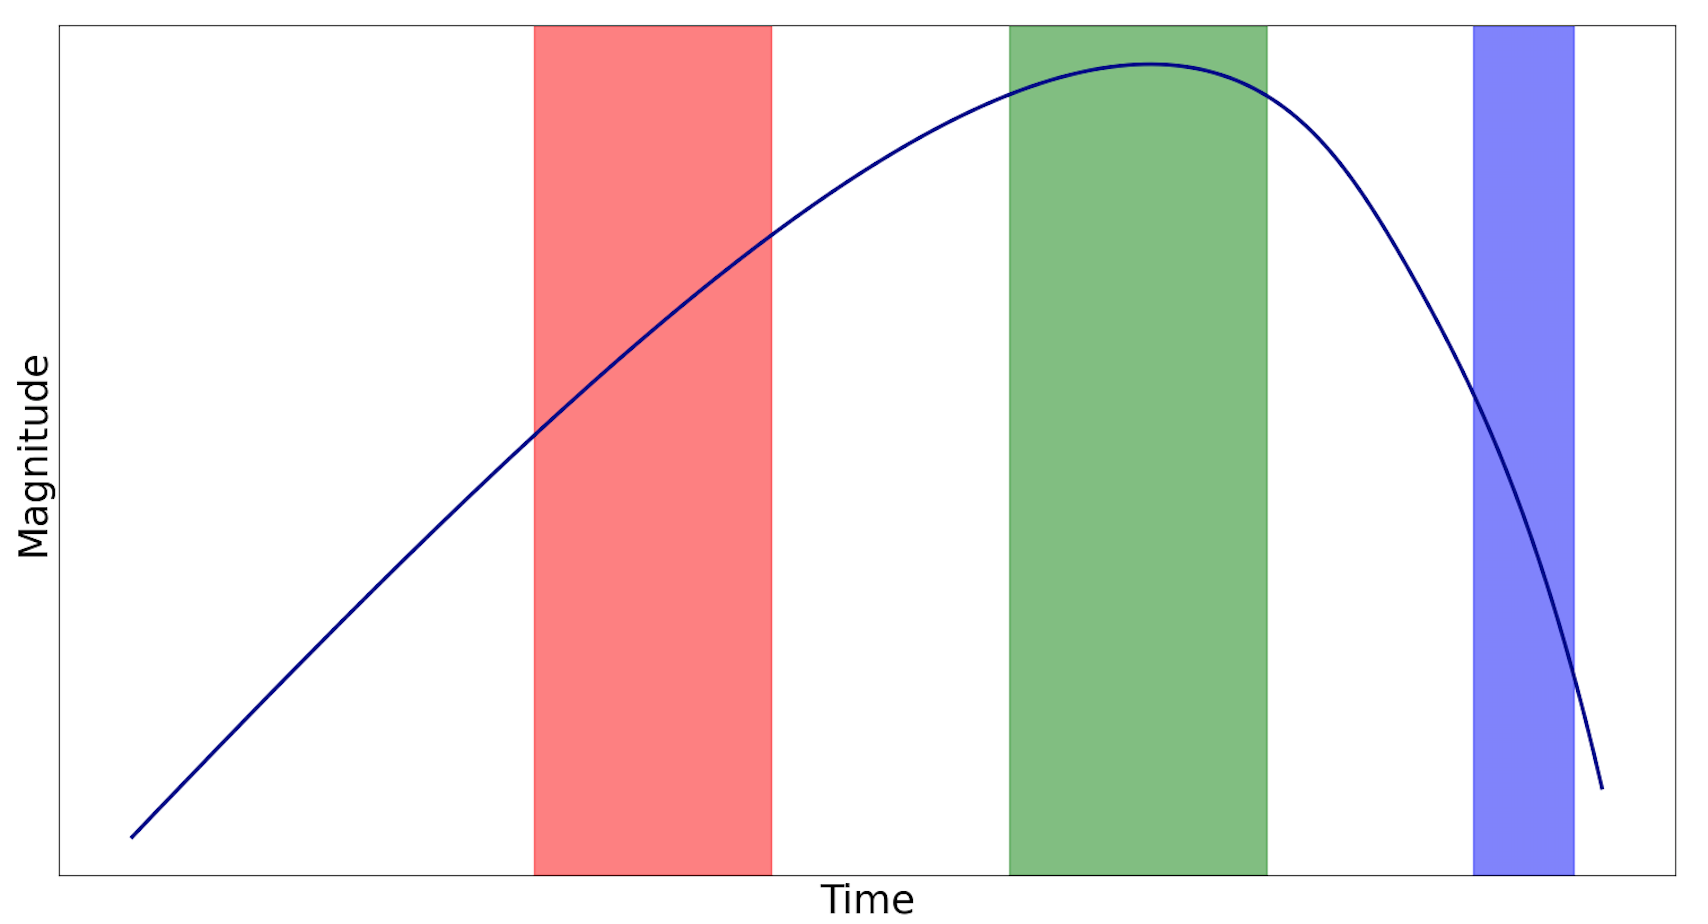
\includegraphics[width=0.5\textwidth]{kilo1.png}
%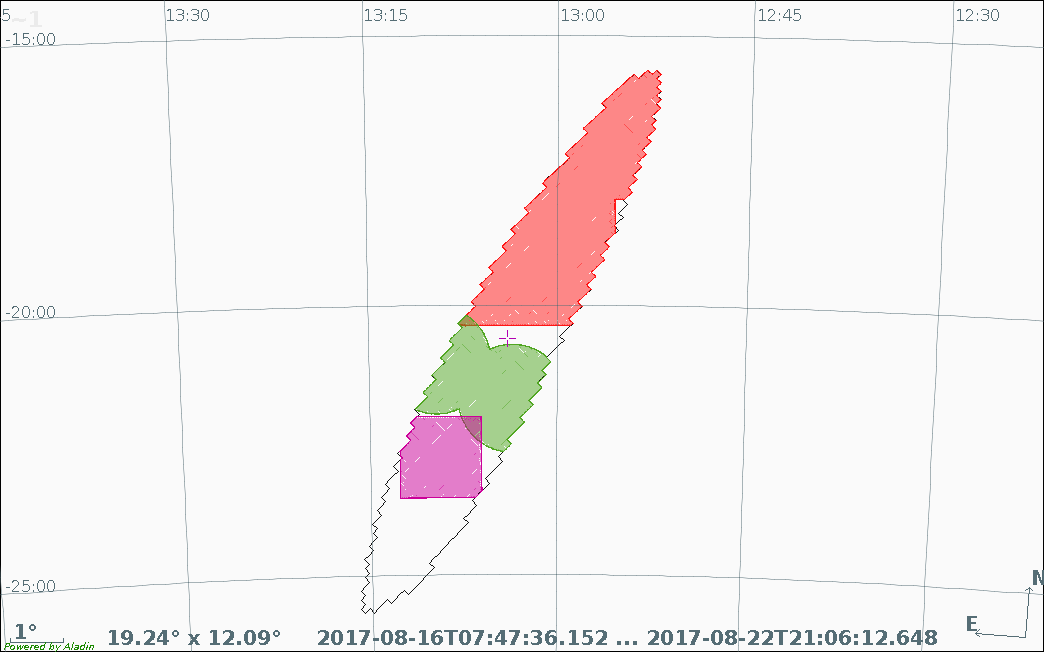
\includegraphics[width=0.45\textwidth]{kilo4.png}
%\caption{A schematic kilonova light-curve, with the
%  associated coverage in time (left panel) and space (right panel).}
%\label{fig:kilonova} 
%\end{center}
%\end{figure}

\subsection{Space and Time MOC: Einstein Telescope and Early Warning Alerts}
The space and time MOC provides us with an effective way to develop new
multi-messenger data analysis tools that will have a crucial role when
the third-generation interferometric gravitational wave observatories,
such as the Einstein Telescope (ET), will begin operation. Here we
figure out a few potential applications. ET will explore the universe
with gravitational waves up to cosmological distances with an
expected detection rate of order $10^{5} - 10^{6}$ black holes and $7\times10^4$
neutron star mergers per year \citep{2020JCAP...03..050M}.
For fast and real time data access, the user can query by a specific
time range the gravitational-wave sky localizations encoded as a space
and time MOC. 

In addition, the ET sensitivity at low frequencies enables enough
signal-to-noise ratio to accumulate before the merger, making possible
a pre-merger gravitational-wave detection and warning for the
electromagnetic/neutrino follow up.  The simulations show that, by
requiring a signal-to-noise ratio $>=$ 12 and a sky localization smaller
than 100 deg$^2$, ET can send an early warning alert between 1 and 20 hours
before the merger (with the mean of the distribution at about 5 hours)
for signals at 40 Mpc \citep{2018PhRvD..97l3014C}. The
electromagnetic/neutrino survey can benefit
in multiple spatial and temporal intersections with a gravitational-wave
sky localization to probe any electromagnetic/neutrino signals temporally
and spatially connected to the inspiral, merger or ring-down phases.
Early warning alerts are also planned in the LIGO-Virgo-KAGRA O4 run with
an experimental capability to produce and distribute early warning
gravitational-wave alerts up to tens of seconds before
merger\footnote{\url{https://emfollow.docs.ligo.org/userguide/early_warning.html}}.  


\subsection{Multi-site positional and temporal search}
Often, a typical query from a virtual observatory (VO) user is to
request all possible records from the VO at a given sky position
and/or at a given time. While this is in principle possible by
dispatching one narrow positional query to every registered Cone
Search, SSA or SIA service and filtering by time, in practice, the
number of queries required leads to an unacceptable load on both
clients and services. Moreover, most of these queries will deliver no
results since most services often lack coverage in the queried
region. If basic footprint/coverage information was available for all
registered services, for instance using VODataService 1.2
\citep{2021ivoa.spec.1102D} only those with coverage in the region
and time of interest would then be queried. This would provide a great
reduction in the number of services to be queried optimizing the
response time. Using the MOC offers the opportunity to provide this
coverage information in a uniform way. The MOC could be stored locally
for a given service or centrally where the coverage for a number of
services would be supported.


\section{MOC principles}

The MOC standard is defined using four basic building blocks:
discretization, unique reference system, hierarchization and efficient
encoding: 

\begin{enumerate}
\item Determine a proper tessellation/discretization methodology for
  each dimension axis (space, time, ...);
\item Fix a unique referential system for each dimension, to avoid 
  reference conversions and thus allowing to easily compare different
  data collections; 
\item Use an hierarchical procedure and a unique representation
  (canonical form) for compacting and quickly manipulating each axis
  coverage at any level of accuracy;
\item Implement at least one serialization in a binary encoding format
  (other serializations are possible, e.g. ASCII). 
\end{enumerate} 

With these principles, a MOC consists of a list of numbers which
represent the indices of the cells mapping the coverage of the spatial
or temporal axis.
As soon as the consecutive cells are used at order n, they will be
hierarchically grouped in their parent cell at order n-1, and
this recursively. This introduces the notion of orders and
associated cell index.
The cell boundary alignment implied by the hierarchical structure
facilitates the combination of cells at different orders. 
To work efficiently on existing hardware, we encode of any pair
(order, index) as a long integer (64 bits), and we reserve the two
most significant bits to encode the type of MOC (spatial, temporal,
or future usages). 
The earlier MOC standard was limited to spatial coverage.
We are reusing these principles to manipulate temporal coverages,
as well as space-time coverages where we can manipulate the two
physical dimensions simultaneously.

\medskip
\par\noindent
We will now explain the conventions chosen for the spatial and temporal axis.

\subsection{Space MOC conventions}
Defining a sky region by a subset of regular sky tessellation or tiles
is not a new idea.  In astronomy, one could find three main methods of
partitioning the sphere : Q3C, HTM and HEALPix which are respectively
using cells in the form of squares, triangles and diamonds for mapping
the celestial sphere.

Several publications have compared these methods \citep{2001misk.conf..638O}. We
justified the choice of HEALPix for the MOC because of these four
points:

\begin{itemize}
\item Equal areas: by construction, HEALPix consists of diamond cells with
  equal spherical surfaces. Thus the area of a given region is trivial
  to compute;
\item Computing time: HEALPix has the peculiarity that the computing
  time does not depend on the hierarchical order \footnote{Note that in the HEALPix
  document orders are refered to as levels, and cells as diamonds.}
  (no recursive  algorithm);
\item Accuracy: HEALPix provides libraries which allow the calculation
  up to accuracy of 0.4 mas (order 29) (\url{http://sourceforge.net/projects/healpix/});
\item Standard: Existence of many HEALPix libraries: C++, Java,
  Fortran, IDL... Also, HEALPix was selected for several all sky
  missions such as WMAP, Planck and Gaia. The HEALPix main web site is
  located at Jet Propulsion Lab (\url{http://healpix.sourceforge.io/}).
\end{itemize}

The HEALPix \citep{2005ApJ...622..759G} tessellation technique divides
the sphere into 12 cells, each of them sub-divided into 4 cells
recursively (see Fig.~\ref{fig:healpix}). Thus the sphere at order 1
will consist of 48 cells,
192 cells at order 2, 768 at order 3 and so on where each cell
at a given order is covering an equal area of the sphere.

\begin{figure}[!htbp]
\begin{center}
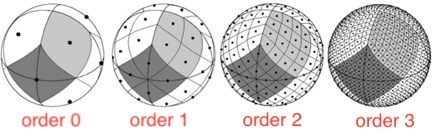
\includegraphics[scale=0.8]{healpix.jpg}
\end{center}
\caption{HEALPix partition of the sphere}
\label{fig:healpix}
\end{figure}

HEALPix allows three coordinate systems: galactic, equatorial and
ecliptic. Allowing various coordinate systems would limit the
possibility to compare efficiently SMOCs. There is indeed no
equivalence between an HEALPix cell described in a given coordinate
system and a cell, or a list of sub-cells expressed in a different
coordinate system. Consequently, the SMOC definition is expressed in
equatorial coordinate using the ICRS reference. This choice has been
motivated by looking at most catalogs and realizing that most of them
are using equatorial coordinates.

To support the encoding based on 64-bit longs, the best resolution
available is provided at order 29 and according to the HEALPix
equations, corresponds approximately to 0.4mas.  The SMOC resolution
is set by the maximum value of the HEALPix order used to define a
region. Its selection depends on the accuracy chosen by the provider
to define the region.  As data set boundaries are not aligned with the
HEALPix cell borders, a SMOC is generally an upper-approximation of
the data set coverage. The quality of this approximation depends
directly on the chosen SMOC resolution (MOCORD\_S).
Table~\ref{table:orders} provides the HEALPix cell angular resolution for
each HEALPix order.

In Figure~\ref{fig:smoc-view} we show the MOC creation, from images to their coverage,
and indicating their corresponding HEALPix numbers. 

\begin{adjustbox}{center,caption={SMOC: from the image
      to the list of numbers based on HEALPix hierarchy tessellation},
    label={fig:smoc-view},nofloat=figure,vspace=\bigskipamount}
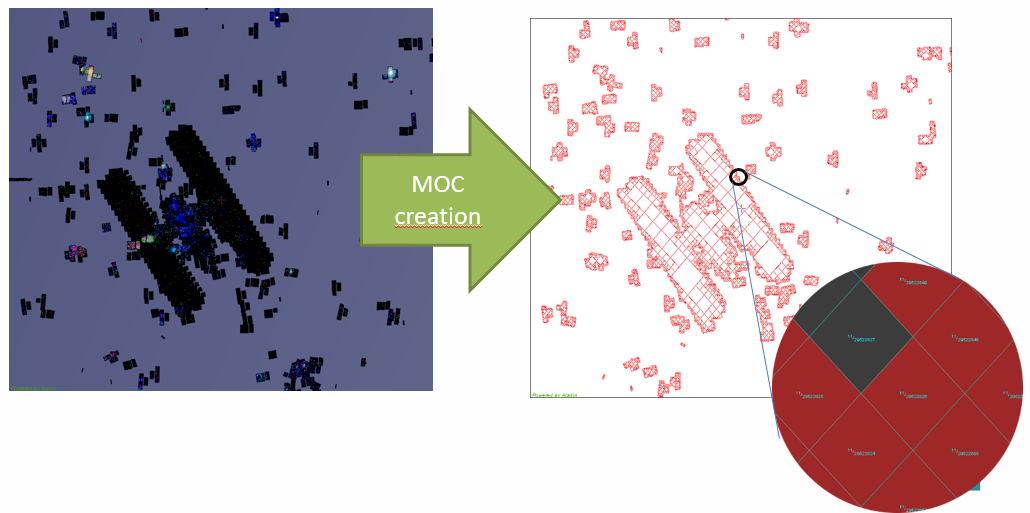
\includegraphics[width=\textwidth]{smoc_view.png}
\end{adjustbox}

\begin{table}[!htbp]
\smallskip
\begin{center}
   {\small
   \begin{tabular} {|l | l| l| l|}
   \hline
   Order & Mean Cell Resolution & Order & Mean Cell Resolution\\
   \hline
   0 	& 	58.63$^{\circ}$ &	15   &       6.442$"$	\\
   1 	& 	29.32$^{\circ}$ &	16   &       3.221$"$	\\
   2 	& 	14.66$^{\circ}$ &	17   &        1.61$"$	\\
   3	&	7.329$^{\circ}$ &	18   &       805.2 mas 	\\
   4	&	3.665$^{\circ}$ &	19   &       402.6   mas	\\
   5	&	1.832$^{\circ}$ &	20   &       201.3 mas	\\
   6 	& 	54.97$^{\prime}$ &	21   &       100.6 mas	\\
   7	&	27.48$^{\prime}$ &	22   &       50.32 mas	\\
   8	&	13.74$^{\prime}$ &	23   &       25.16 mas	\\
   9	&	6.871$^{\prime}$ &	24   &       12.58 mas	\\
   10	&	3.435$^{\prime}$ &	25   &        6.291 mas	\\
   11	&	1.718$^{\prime}$ &	26   &       3.145 mas	\\
   12 	& 	51.53$"$ &		27   &       1.573 mas	\\
   13	&	25.77$"$ &		28   &       786.3 $\mu$as	\\
   14	&	12.88$"$ &		29   &       393.2 $\mu$as	\\
   \hline
   \end{tabular}
   }
\caption[SMOC order and cell resolutions]{SMOC cell resolutions for each order. The SMOC HEALPix cell has
  constant area, not constant linear dimensions.}\label{table:orders}
\end{center}
\end{table}


\begin{table}[!htbp]
\smallskip
\begin{center}
   {\scriptsize
   \begin{tabular} {|l | l| l| l| l|}
   \hline
   Order & Time Cell Resolution ($\mu$s)  & Order & Time Cell Resolution ($\mu$s) \\
   \hline
0       &       2305843009213693952 ($\simeq$73117.8y) 	& 31   & 1073741824 ($\simeq$17.9m) \\
1       &       1152921504606846976 ($\simeq$36558.9y) 	& 32   & 536870912 ($\simeq$9m) \\
2       &       576460752303423488 ($\simeq$18279.4y)	& 33   & 268435456 ($\simeq$4.5m) \\
3       &       288230376151711744 ($\simeq$9139.7y)	& 34   & 134217728 ($\simeq$2.2m) \\
4       &       144115188075855872 ($\simeq$4569.9y)	& 35   & 67108864 ($\simeq$1.1m) \\
5       &       72057594037927936 ($\simeq$2284.9y)	& 36   & 33554432 ($\simeq$33s) \\
6       &       36028797018963968 ($\simeq$1142.5y)	& 37   & 16777216 ($\simeq$16s) \\
7       &       18014398509481984 ($\simeq$571.2y)	& 38   & 8388608 ($\simeq$8s) \\
8       &       9007199254740992 ($\simeq$285.6y)	& 39   & 4194304 ($\simeq$4s) \\
9       &       4503599627370496 ($\simeq$142.8y)	& 40   & 2097152 ($\simeq$2s) \\
10      &       2251799813685248 ($\simeq$71.4y)	& 41   & 1048576 ($\simeq$1s) \\
11      &       1125899906842624 ($\simeq$35.7y)	& 42   & 524288 ($\simeq$524ms) \\
12      &       562949953421312 ($\simeq$17.8y)		& 43   & 262144 \\
13      &       281474976710656 ($\simeq$8.9y)		& 44   & 131072 \\
14      &       140737488355328 ($\simeq$4.5y)		& 45   & 65536 \\
15      &       70368744177664 ($\simeq$2.2y)		& 46   & 32768 \\
16      &       35184372088832 ($\simeq$1.1y)		& 47   & 16384 \\
17      &       17592186044416 ($\simeq$203.6d)		& 48   & 8192 \\
18      &       8796093022208   ($\simeq$101.8d)	& 49   & 4096 \\
19      &       4398046511104 ($\simeq$50.9d)		& 50   & 2056 \\
20      &       2199023255552 ($\simeq$25.4d)		& 51   & 1024 \\
21      &       1099511627776 ($\simeq$12.7d)		& 52   & 512 \\
22      &       549755813888 ($\simeq$6.3d)		& 53   & 256 \\
23      &       274877906944 ($\simeq$3.2d)		& 54   & 128 \\
24      &       137438953472 ($\simeq$1.6d)		& 55   & 64 \\
25      &       68719476736 ($\simeq$19.1h)		& 56   & 32 \\
26      &       34359738368 ($\simeq$9.5h)		& 57   & 16 \\
27      &       17179869184 ($\simeq$4.8h)		& 58   & 8 \\
28      &       8589934592 ($\simeq$2.4h)		& 59   & 4 \\
29      &       4294967296 ($\simeq$1.5h)		& 60   & 2 \\
30      &       2147483648 ($\simeq$35.8m)		& 61   & 1 \\
   \hline
   \end{tabular}
   }
\caption[TMOC order and cell resolutions]{TMOC cell resolutions for each orders.}\label{table:tmocorders}
\end{center}
\end{table}


\subsection{Time MOC conventions}
\label{sec:tmoc1}


In order to represent time coverage, we need to select a-priori the
total range of time that we will cover with the notation. Following
the same SMOC principles, we need to use a discrete time axis where
each unit element of this axis has a constant duration. We adopt
the Julian Date convention, very common in astronomy and a nominal
resolution of 1$\mu$s. The temporal dimension being by nature 1D unlike
the spatial dimension, we opt for a order progression by factor of
2 (4 for SMOC) and therefore 62 orders (30 for SMOC). This way we
can address $2^{62}$ cells in an unsigned 64-bit integer,
i.e. a little bit more than 73000 years at
1$\mu$s resolution, enough for most astronomical time events. At the
deepest order (61) the TMOC cell number is the number of $\mu$s since
JD=0.

The time is a relative observation, and depends on the position of the
observer. There are many time scales for measuring time:
Terrestrial Time (TT), Barycentric Coordinate Time (TCB), Geocentric
Coordinate Time (TCG), Ephemeris Time (ET), Barycentric Dynamic Time
(TDB), International Atomic Time (AI), etc. We opt for the TCB
reference (see \cite{2015A&A...574A..36R} for details). Our
choice is motivated by the fact that this system is linear by
construction and has been adopted by numerous missions such as Gaia.

It may be necessary to convert the temporal events to the
chosen scale. If the ephemeris required for this conversion are
not available, opt to degrade the accuracy of the time measurement
(typically around 20 minutes for observations within the Earth orbit
environment to cover all possible observer positions).
Table~\ref{table:tmocorders} is showing some time values at a given order.

In Figure~\ref{fig:tmoc-view} we show the creation of TMOC, from a time
series to the list of numbers based on time discretization.
      
\begin{adjustbox}{center,caption={TMOC: from the
      time series to the list of numbers based on time
      discretization},label={fig:tmoc-view},nofloat=figure,vspace=\bigskipamount}
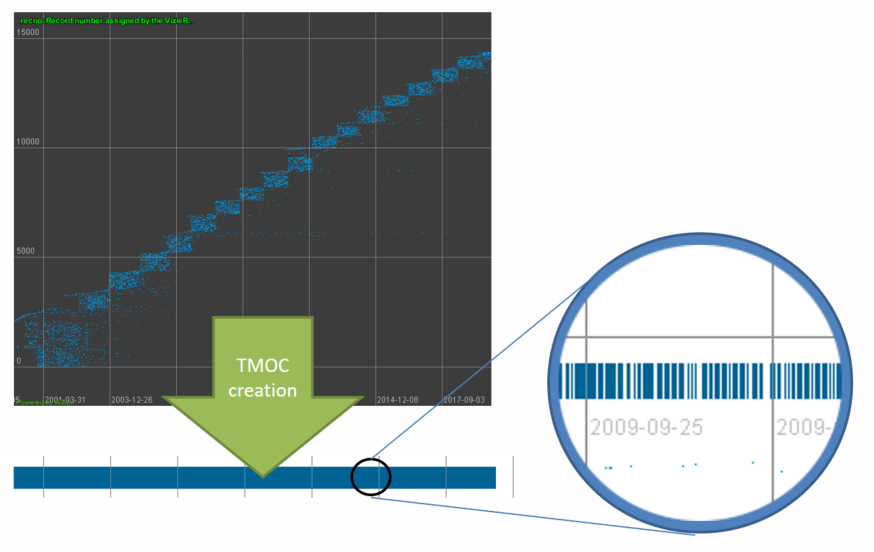
\includegraphics[width=\textwidth]{tmoc_view.png}
\end{adjustbox} 

\subsection{Space and Time MOC conventions}
To respond to the different use cases presented at the beginning of
the document, the SMOC and TMOC independently are not enough. We need
to link the two dimensions in a global mechanism. In other words, we
need to be able to select the SMOC using a time window or to select a
TMOC using a spatial constraint. Implementing this linkage would allow
the potential users to select and interact with the astronomical
collections which support space and time and use logical
operators between them.

Our approach is to combine these two dimensions - time and space - by
associating each time period (coded according to the TMOC
convention) with its spatial region (coded according to the SMOC
convention). For that, we interleave the information of time coverage
with the information of space coverage for this period.

This two-dimensional interleaving approach has the advantage of making
the resolutions chosen for time and for space independent. For
instance, it is possible to describe observation coverage with a low
resolution for time while using a high spatial
resolution.
A single coding for indexing space and time simultaneously would imply
at best very low resolution MOCs due to the 64-bit coding constraint. 
We thus proposed the interleaving algorithm which allows us to define and
manipulate high resolution STMOCs of reasonable sizes for fast algorithms
(see Appendix~\ref{app:perf} for STMOC performance).
In Figure~\ref{fig:stmoc-view} we show the visual representation of an STMOC,
in which at a given TMOC range we obtain the corresponding SMOC. 
 
\begin{adjustbox}{center,caption={STMOC visual representation in which
      at a given TMOC range we obtain the corresponding SMOC},
    label={fig:stmoc-view},nofloat=figure,vspace=\bigskipamount}
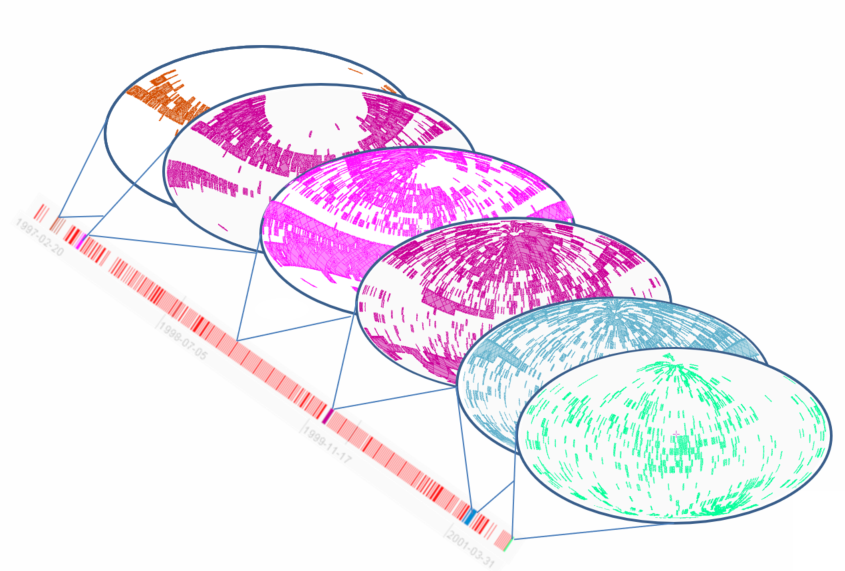
\includegraphics[width=0.8\textwidth]{stmoc_view.png}
\end{adjustbox}

\section{SMOC and TMOC encoding}
The encoding described in this section guarantees backward compatibility
with MOCs corresponding to previous versions of this standard.

\subsection{Space MOC or SMOC}
As introduced above, the SMOC {\bf should} be based on the
HEALPix tessellation of the sphere, expressed in the ICRS coordinate
reference system for celestial coverages. This document does not describe
the use of SMOC outside celestial scope. However, it is possible to use
SMOC for other coverages, such as planetary coverages. The definition of
the unique reference for each body will have to be defined. Two complementary
encoding formats are defined: a string serialization based on ASCII and a
binary format based on FITS.

\subsubsection{Numbering}

The numbering scheme used in SMOC for specifying the cell indices {\bf
  must} follow the "NESTED" HEALPix numbering schemes
\citep{2005ApJ...622..759G}. This numbering consists of enumerating all cells in a
specific order. For instance, at order 1, there are 48 cells (12x4)
enumerated from 0 to 47. In this scheme, the 4 sub-cells of cell M
have the indices: (M$\times4)+3$, (M$\times4)+1$, (M$\times4)+2$,
(M$\times4$) in reading
order. And reciprocally, the parent index of cell N is
N/4. Each SMOC cell is coded by a pair of numbers:
(order, index) which are the HEALPix order and the HEALPix index in this
order.

\begin{adjustbox}{center,caption={HEALPix numbering principle},
    label={Fig:HEALPix numbering},nofloat=figure,vspace=\bigskipamount}
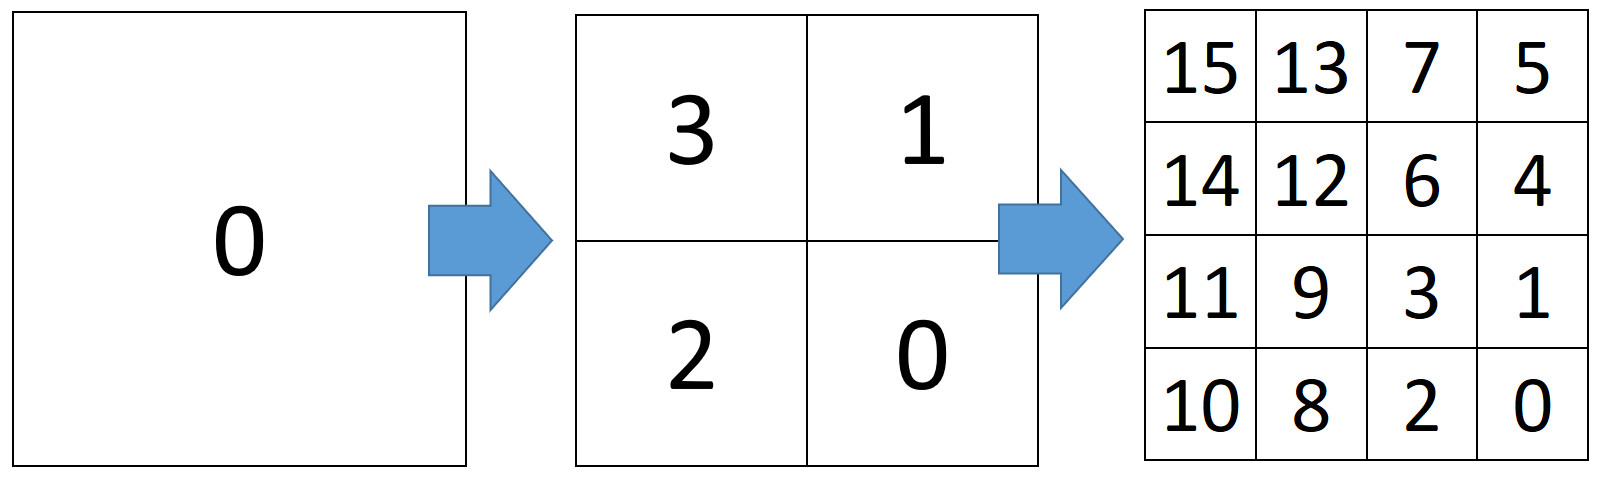
\includegraphics[width=\textwidth]{nested_healpix.jpg}
\end{adjustbox}

{\bf Note:} The order 0 is a special case, it contains only 12
cells enumerated from 0 to 11.


\subsubsection{Sky coordinates}
The mechanism used to determine which HEALPix cell contains a given
sky location is described in the main article defining the HEALPix
system \citep{2005ApJ...622..759G}. Several support libraries
supporting the most important set of primitives are already available.
These libraries are required if one wants to generate SMOCs, and also
wants to compare them with sky coordinates. Though please
note that these libraries do not have built-in support to performing
basic SMOC arithmetics.

\subsection{Time MOC or TMOC}
As introduced above, TMOC {\bf must} be based on JD system, the time
scale TCB, and the Solar System Barycenter as the reference
position \citep[see also][]{2019ASPC..523..497F} and section~\ref{sec:tmoc1}.
The best resolution supported by TMOC is $1 \mu$s.

In the case that the time scale and the time reference position are unknown,
we recommend to set the time resolution of the generated TMOC to order
31, e.g. about 1000 seconds (see Table~\ref{table:tmocorders}) corresponding
to about twice the light travel time correction between the Earth and
the Solar Barycenter. Please refer to the VO note on TIMESYS for more
information about this limitation \citep{timesysnote}.


\subsubsection{Numbering}
The numbering scheme used in TMOC for specifying the time cell indices
{\bf must} reuse a similar hierarchical principle as for the SMOC
with the difference that the time line has only one dimension, so the
hierarchical progression uses a factor of 2 instead of 4, and there is
no need to use a HEALPix mapping.

TMOC has 62 orders, and at the best
resolution (order 61), a time event will be coded by the integer value
representing the number of $\mu$s of this event since JD=0.

Two consecutive cells at order N with the indices
  (M$\times$2)+1, (M$\times$2) will be coded at order N-1 with the index
  M and thus recursively. The order N-1 cell duration is 2 times more 
  than the N cell duration (61: 1 $\mu$s, 60: 2 $\mu$s, 59: 4 $\mu$s, etc...).

\subsection{Serialization}
A MOC can be manipulated and serialized either as a list of cell
numbers for each order (hierarchical view), or as a list of intervals
at the deepest order (range view). These two methods are used for
SMOC, TMOC and STMOC serializations and are presented below.

\subsubsection{Binary serialization}
To encode a MOC in a FITS file, each MOC pair (order, index) {\bf
  must} be stored in a FITS binary table. Two packaging modes are
defined: either all MOC pairs (order, index) are stored individually
thanks to NUNIQ packaging, or all ranges of indices at the deepest
order are stored following the RANGE packaging.

\paragraph{NUNIQ Packaging (valid for SMOC only)}
The NUNIQ scheme defines an algorithm for packaging a MOC pair (order,
index) into a single integer for compactness:
$$
    \textit{uniq} = 4 \cdot (4\,^\textit{order}) + \textit{index}
$$

\par\noindent
The inverse operation is:
\begin{eqnarray*}
    \textit{order} & = &\log_2(\textit{uniq}/4)/2\\
    \textit{index} & = &\textit{uniq} - 4 \cdot (4\,^\textit{order})
\end{eqnarray*}

\par\noindent The list of cells {\bf must} be well-formed
(see Section~\ref{sec:can}) allowing
to express both hierarchy or range representation. The resulting
list is stored in a single-column binary table extension.
For orders strictly lower than 14 these UNIQ values can be stored
in a 32-bit signed integer (TFORM1='J') , and for the higher
orders in a 64-bit signed integer (TFORM1='K').

\paragraph{RANGE packaging}
For the coding of RANGE alternative packaging, all the indices are
expressed at the maximum resolution, and it is the succession
of intervals that will be stored in the FITS table as 
two 64-bit signed integers (TFORM1='K') :
the smallest index of the interval and the index strictly greater
than the largest value of the interval. The RANGE values {\bf must}
be in ascending numerical order. The resulting list is stored in a
single-column binary table extension. 


\paragraph{Backward compatibility}
RANGE packaging has been introduced for MOC2.0.
This method is generally faster than the previous one for reading or
writing a MOC because the internal representation of MOC
in memory is often range oriented. However, we recommend to
use the first method for SMOC for compatibility with existing libraries 
not yet compatible with MOC2.0.

\subsubsection{ASCII serialization}
To encode a MOC as a string each MOC pair (order, index) {\bf must} be written
sequentially in an ASCII stream as two ASCII numbers separated
by slash ("/": decimal ASCII code 47). The order and the slash prefix
{\bf may} be omitted if the previous cell has the same order. The
elements are separated by one or several space characters (space, CR,
LF) corresponding respectively to the decimal ASCII codes: 32, 13, and
10.

The usage of a range operator is allowed in the list of indices using the
dash ("-": decimal ASCII code 45) as a separator: lowindex-highindex.
The list of cells {\bf must} be well-formed, and the values {\bf must}
be in ascending numerical order.

If the best resolution of the MOC (moc order) is greater than the
greatest stored order, the moc order {\bf must} be provided, followed
by a slash ("/") without any associated index value.
In the following example all the
cells underneath the explicit pair (order, cell) are implicitly covered
up to order 8, the moc order, annotated followed by the terminator "/".
Without the terminator we would only have the information of the explicit
pair (order, cell), and the assumed best resolution would be at order 2.   


\paragraph{Example of an ASCII MOC:}
\begin{lstlisting}[]
    1/1 2 4 2/12-14 21 23 25 8/
\end{lstlisting}

\begin{center}
  {\small
  \begin{tabular} { l l l l l l l l l }
   & 1/1   & 2  & 4  & 2/12-14 & 21 & 23 &  25 & 8/ \\
   & $\downarrow$ & $\downarrow$ & $\downarrow$ & $\downarrow$ & $\downarrow$ & $\downarrow$ & $\downarrow$ & $\downarrow$ \\
Order:     & 1    & 1 & 1 & 2        & 2  &  2 & 2  & 8 \\
Cell:      & 1    & 2 & 4 & 12 to 14 & 21 & 23 & 25 & \\
\end{tabular}}

MOC ASCII encoding
\end{center}


\paragraph{EBNF definition of an ASCII MOC:}
\begin{lstlisting}[]
  smoc  ::= 's'? moc
  tmoc  ::= 't'? moc
  stmoc ::= ('t' moc 's' moc)+
  moc ::= ordval (sep+ ordval)* [sep+ order]
  ordval ::= order sep* vals
  order ::= int '/'
  vals ::= val (sep+ val)*
  val ::= int | (int '-' int)
  sep ::= [ \n\r]
  int ::= [0-9]+
\end{lstlisting}
Note that we use Extended BNF supporting regular expression
syntax with the following rules: i) postfix * means "repeated
0 or more times”; ii) postfix + means "repeated 1 or more
times”; iii) postfix ? means "0 or 1 times". The first three
rules depend on the MOC type, i.e. SMOC for space, TMOC for
time and STMOC for space-time. 

\section{STMOC encoding}
\label{sec:stmoc}
Coding STMOC consists in the following: for each element of a
temporal coverage we list the associated spatial coverage using the
natural packaging as defined in the previous section. 

\subsection{ASCII Serialization}
The ASCII serialization of a STMOC is a string following the ASCII MOC
serialization presented below, which interleaves time coverage as a
excerpt of TMOC and associated space coverage as a SMOC. Each TMOC
element {\bf must} be prefixed by the character 't', and each SMOC
element {\bf must} be prefixed by the character 's'.
The character is thus omitted until the next dimension element is
defined.

\paragraph{Example of an ASCII STMOC:}
\begin{lstlisting}[]
  t61/1 s29/0-2 t61/3 s28/0 t60/2 61/6 s29/2 5
\end{lstlisting}

\begin{center}
{\small
  \begin{tabular} { l l l l l l l l l }
   & t61/1      & s29/0-2    & t61/3      & s28/0 & t60/2 & 61/6 & s29/2 & 5\\
   & $\downarrow$ & $\downarrow$ & $\downarrow$ & $\downarrow$ & $\downarrow$ & $\downarrow$ & $\downarrow$ & $\downarrow$ \\
Dimension: & Time & Space  & Time  & Space & Time  & (Time) & Space & (Space) \\
Order:     & 61   & 29     & 61    & 28    & 60    & 61     &  29   & (29)\\
Cell:      & 1    & 0 to 2 & 3     & 0     & 2     & 6      &  2    & 5 \\
\end{tabular}}
STMOC ASCII encoding: two independent numbering. Values in parenthesis are implicit from the previous encoding substring.
\end{center}

\subsection{Binary Serialization}
The binary serialization of a STMOC is a FITS binary table following
the RANGE packaging presented previously, which interleaves time range(s)
and their corresponding space coverage ranges. Following the binary
RANGE serialization method described below, each range (time or space)
is coded as two 64-bit signed integers ([min..max[). To distinguish time
and space indices, the time indices {\bf must} have the 64th bits forced
to 1. It is not a sign inversion (two's complement) but a mask affecting
only that last bit without touching any other bits.  The order of
dimensions is always time first.

\paragraph{Illustration of STMOC interleaving method}
\begin{adjustbox}{center,caption={STMOC encoding with two independent
      numbering system},
    label={fig:stmocbin-encoding},nofloat=figure,vspace=\bigskipamount}
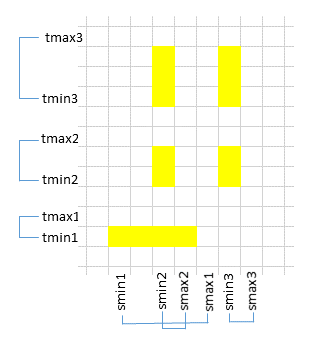
\includegraphics[width=0.5\textwidth]{STMOCbin.png}
\end{adjustbox}

\par\noindent
This list of ranges will be  coded in a list of 64bits integers
(time indices with the 64th bit forced to 1) as:
\begin{lstlisting}[]
   tmin1 tmax1 smin1 smax1 tmin2 tmax2 tmin3 tmax3 smin2 smax2 smin3 smax3
\end{lstlisting}

STMOC encoding must conform to the following simple rules:
\begin{itemize}
\item{Temporal cells which are sequential and have the SAME
  spatial coverage MUST be aggregated in the coding scheme.}
\item{The cell order MUST also be increasing first on the
  temporal axis, then on the spatial axis.}
\end{itemize}


\section{FITS keywords}
\label{sec:fits-key-moc} 
For the binary representations which are packaged in binary FITS table,
we define a set of FITS keywords, their possible values and set when
those fields are required, optional or recommended in
Table~\ref{table:fits_stmoc} and show an example of FITS headers for a MOC.
Since MOC~1.1 \citep{2019ivoa.spec.1007F} the {\tt PIXTYPE = "HEALPIX"}
keyword/value is no longer required, and should be omitted. 
The keyword {\tt MOCORDER} is no longer required either, but it can be used for
backwards compatibility if required.
Other FITS Keywords could be used to augment the information like DATES and ORIGIN. 
 
\begin{table}[!htbp]
\smallskip
\begin{center}
   {\small
   \begin{tabular} {|l | p{6cm}| c| c|}
   \hline
   {\bf Keyword} & {\bf Definition} & {\bf MOC1.1} & {\bf MOC2.0} \\
   \hline
   MOCVERS  & The version of the MOC encoding standard. If it is following this document (TMOC, STMOC and STMOC), it {\bf must} be '2.0'. If not defined it is assumed to be 1.1. & NA & mandatory \\
   MOCDIM	    & Physical(s) dimension(s). Either 'SPACE' for SMOC, 'TIME' for TMOC or 'TIME.SPACE' for STMOC. If omitted, 'SPACE' is assumed for backward compatibility. & NA & mandatory \\
   ORDERING & The packaging method used. It is either NUNIQ (V1.1 or V2.0 SMOC) or RANGE (V2.0). & mandatory & mandatory \\
   COORDSYS & The coordinate system in use. The value {\bf must} be 'C' for SMOC (ICRS). & mandatory & mandatory  \\
   TIMESYS  &  The time system in use. The value {\bf must} be 'TCB' for TMOC.  & NA & mandatory \\
   MOCID    & Original data identifier. If the original data set has been declared in the VO registry [11]\citep{2020arXiv200707519D}, we strongly encourage to use the IVOA identifier (ex: "ivo://wfau.roe.ac.uk/twomass-dsa"). & optional & optional \\
   MOCTOOL  & The name of the MOC software generator. It is also recommended to add the software version number to its name. & optional & optional \\
   MOCTYPE  & Provenance data type. Either 'IMAGE', or 'CATALOG'. In the first case for areas computed from existing images and/or footprint or even STC strings, in the second case for areas computed from a collection of point sources using a unique and/or derived area. & optional & optional \\
   MOCORD\_S  & Best resolution of the space dimension, expressed as the order. & NA & mandatory\\
   MOCORD\_T  & Best resolution of the time dimension, expressed as the order. & NA & mandatory \\
   \textit{MOCORDER} & Best resolution of the space dimension, expressed as the order. & mandatory & NA \\
   \textit{PIXTYPE} & 'HEALPIX'  & mandatory & NA \\
   \hline
   \end{tabular}
   }
\end{center}
\caption{FITS Keywords for MOC.}
\label{table:fits_stmoc}
\end{table}

 
%\clearpage 
\paragraph{Example of FITS headers for a MOC:}
\par\noindent
\begin{lstlisting}[basicstyle=\footnotesize\ttfamily]
SIMPLE   =                      T
BITPIX   =                      8
NAXIS    =                      0
EXTEND   =                      T
END
    
XTENSION = 'BINTABLE'            / HEALPix Multi Order Coverage map
BITPIX   =                      8
NAXIS    =                      2
NAXIS1   =                      4
NAXIS2   =                  16461
PCOUNT   =                      0
GCOUNT   =                      1
TFIELDS  =                      1
TFORM1   = '1J      '
TTYPE1   = 'UNIQ    '            / HEALPix UNIQ pixel number
ORDERING = 'NUNIQ   '            / NUNIQ coding method
COORDSYS = 'C       '            / ICRS reference frame
MOCDIM   = 'SPACE   '            / Physical dimension
MOCORD_S =                    12 / MOC resolution (best order)
MOCTOOL  = 'Aladin11.1'          / Name of the MOC generator
MOCTYPE  = 'CATALOG '            / Source type (IMAGE or CATALOG)
MOCID    = 'ivo://CDS/I/259'     / Identifier of the collection
MOCVERS  = '2.0     '            / MOC standard version
ORIGIN   = 'ivo://CDS'           / MOC origin
DATE     = '2013-06-15T11:50:43' / MOC creation date
EXTNAME  = 'Tycho MOC'           / MOC name
END
\end{lstlisting}

\section{MOC usage constraints}

\subsection{Canonical form}
\label{sec:can}
The speed of MOC operations - creation, union, intersection, etc
is directly dependent on the speed of the equality test. It is
therefore essential to always express a MOC in a canonical way, ie
one unique representation for one coverage. Thus in the case of a
hierarchical representation a MOC \textbf{must} be "well-formed", i.e. 
redundant cells are not allowed, the cells must be ascending sorted
and the hierarchical encoding principle must be respected. Thus it
is not allowed to encode sibling cells instead of their parent (4
siblings for SMOC, 2 siblings for TMOC). In the case of range
representation, the list of ranges must be expressed without
overlapping and sorted ascending.


\subsection{Compromise of Volume VS. Resolution}
In order to easily handle MOCs, it is recommended to adjust
the maximum resolution, i.e. the deepest order, to obtain a representation of
the desired data volume even if it means degrading the accuracy of the coverage
(see Appendix~\ref{app:perf}). In the case of STMOC, it is possible to adjust
the spatial order and/or on the temporal order independently.

\subsection{Working resolution}
The MOC has been designed to be able to efficiently handle observation
coverages (images, catalogs, ...). During the construction of the
MOC, we must then ensure that at the chosen nominal resolution, any cell
of the MOC contains at least one observation (no empty cell). To keep
this assumption, during operations (unions, intersections ...)
between 2 or more MOCs (e.g: MocA $\cup$ MocB $\cup$ MocC) of different
resolutions, the operations
must always be done at the worst (lowest) resolution of the original MOCs
in order not to lose any observations, nor to create empty cells (see
Figure \ref{fig:operation}), and finally to guarantee the set logical
properties (commutativity, associativity,...).

\begin{figure}[!htbp]
\begin{center}
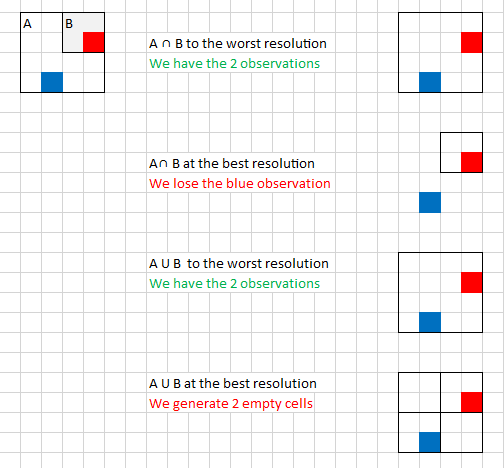
\includegraphics[scale=.5]{operation.png}
\end{center}
\caption[Visualisation of MOC operations]{Visualisation of the
  principles behind MOC operators}
\label{fig:operation}
\end{figure}

%However, MOC can also be used to manipulate surfaces, unrelated to
%observations. When used this way, nothing prevents working at the best
%resolution and some operations such as oversampling, dilation,
%erosion may be applied.
Note that MOC usage can be diverted to also manipulate surfaces unrelated
to observations. When it is used this way such operations (oversampling,
surface dilatation or surface erosion) can be applied. 
And in this context it is necessary to work at the best (highest)
resolution of the involved MOCs for preserving the properties of the
surfaces operations (commutativity, associativity, ...).




\section{Summary and conclusion}
We have reviewed the standards for encoding the different MOC flavors,
the space MOC (already described in version 1.1 of this document),
SMOC, the time MOC, TMOC and the space-time MOC, STMOC. 
The conventions for space and time MOC are the following:
\begin{itemize}
\item The SMOC is simply defined as a list of HEALPix indices (order, index).
\item According to HEALPix, the sphere is divided in cells,
  hierarchically grouped 4 by 4 with 30 orders and the space coverage
  for the deepest order is approximatively 0.4mas.
\item The space reference system is ICRS. 
\item The TMOC is simply a list of time interval indices (order, index).
\item The time scale is divided in intervals hierarchically grouped 2 by
  2 with 62 orders and the time coverage for the deepest order is 1 $\mu$s. 
\item The time values are defined using JD = 0 as the origin, in Barycentric system. 
\end{itemize}

Once defined and encoded for a given astronomical collection, one
can easily combine the MOCs for these two dimensions to create a
merged STMOC which can be used to navigate and access the collection
through their coverage for both time and space simultaneously.
The possibilities are then very interesting and will be a very
valuable astronomical tool.

\bibliography{ivoatex/ivoabib,ivoatex/docrepo,moc}


\appendix
\section{Version History}

\subsection{Changes between versions 1.1 and 2.0}

The differences between version 2.0 of MOC and the preceding version 1.1 are:
\begin{itemize}
   \item The adaptation of the previous MOC (spatial) to a temporal
     dimension;
   \item The definition of the concept of MOC allowing to handle both
     spatial and temporal MOCs;
   \item The extension of ASCII and binary coding to support these new
     concepts.
    \item Relax the language to allow a future use of MOC with a non-sky coordinate system. 
\end{itemize}
Taking these extensions into account required a major restructuring of
the document.

\subsection{Changes between versions 1.0 and 1.1}
The differences between version 1.1 of MOC and the preceding version
1.0 are:
\begin{itemize}
   \item The String MOC serialization was moved from an informative
     section (suggested syntax) to the normative section;
   \item A MOCORDER convention for String SMOC and JSON SMOC was added.
     \citep{2020arXiv200707519D}.
\end{itemize}

\section{Suggested algorithms for basic operations}
Mapping a MOC to a unique sorted list of cells at the deepest
resolution order allows usage of very easy and very fast
algorithms. Basic operations such as unions or intersections can be
computed via bit shifts and simple dichotomic algorithms on sorted
lists.  To reduce as much as possible the memory requirement, a good
practice is to store range sets of continuous cells [minValue
  .. maxValue[, instead of individual cells.

\subsection{Union: moc1 $\cup$ moc2}
\begin{lstlisting}
   Map moc1 to rangeList
   Map moc2 in the same rangeList
   Unmap the resulting rangeList
\end{lstlisting}

\subsection{Intersection: moc1 $\cap$ moc2}
\begin{lstlisting}
   Map moc1 in rangeList1
   foreach order/index of moc2
        shift=2*(maxOrder-order)
        append in a rangeList2 the intersection between
              [index << shift .. index+1 << shift[
        and   the corresponding range(s) of rangeList1
   Unmap rangeList2
\end{lstlisting}

\subsection{Map: moc To rangeList}
\begin{lstlisting}
   foreach order/index of moc
         shift=2*(maxOrder-order)
         append in rangeList [index << shift , (index+1) << shift[
         (the range overlapping must be adjusted)
\end{lstlisting}

\subsection{Unmap: rangeList To moc}
\begin{lstlisting}
   for order = 0 to maxOrder
      end if rangeList is empty
      shift = 2*(maxOrder-order)
      offset = (1<<shift) -1
      foreach range [min..max[ of rangeList
         append in moc order/index where index is in [m1 .. m2[
               m1 = (min+offset) >> shift
               m2 = max >> shift
         remove from rangeList [m1<<shift .. m2<<shift[
\end{lstlisting}

\section{Basic HEALPix functions}
For generating space MOC from observations, or drawing them on the
sphere, an HEALPix library is required. The basic functions available
in all HEALPix libraries are the following :
\begin{itemize}
   \item npix <= coordToNpix(order, alpha,delta) : returns the HEALPix
     cell index containing the alpha,delta coordinates.
   \item ArrayOfNpix <= queryDisc(order, alpha,delta,radius) : returns
     the list of cell indices covering the (long,lat,radius) cone
   \item ArrayOfNpix <= queryPolygon(order, alpha1,delta1, $\cdots$
     alphaN,deltaN): returns the list of cell indices covering the
     spherical polygon
   \item (alpha,delta) <= NpixToCoord(order,npix) : returns the
     coordinates of the center of order/npix cell.
   \item ArrayOf(alpha,delta) <= NpixToCorners(order,npix) : returns
     the corner coordinates of order/npix cell.
\end{itemize}

\section{Basic time functions} 
For generating TMOC from observations, a time library might be required
to convert the dates are not expressed in JD TCB
\begin{itemize} 
\item \url{http://www.iausofa.org/}
\item \url{http://javastro.github.io/jsofa/}
\item \url{https://docs.astropy.org/en/stable/time/#module-astropy.time}
\item Obtain the index from the JD: calculating the TMOC index from
  a JD expressed as a double can be done by simple multiplication,
  but will only allow millisecond accuracy around the present time
  because of the conversion from double to long. 

\begin{lstlisting}[language=C]
    long getMicrosec(double jd) {
        return (long)(jd*86400000000L);
    }
\end{lstlisting}

To guarantee microsecond accuracy, a solution may be to use a second 
parameter to indicate an origin expressed as a long integer from JD=0,
close to the observation dates, and to use the offsets of these
observations, expressed as double, from this new origin.

\begin{lstlisting}[language=C]
    long getMicrosec(double offset, long origin) {
        long x = (long)(offset*86400000000L);
        return x + (origin*86400000000L);
    }     
\end{lstlisting}

%\begin{lstlisting}[language=C]
%static public long getMicrosec(double jd, long offset) {
%    long micron = (long)(jd*DAYMICROSEC);
%    return micron + (offset*86400000000L);
%}
\end{itemize} 

\section{MOC Volume and Performances}
\label{app:perf}
The MOC describes ranges of space and time as an explicit list of cells. The
volume can vary a lot from a few bytes to several megabytes.
Since MOC is hierarchical, its volume mainly depends on three factors:
\begin{itemize}
\item The chosen STMOC resolutions (spatial and temporal).
\item The geometry of the region and its time coverage.
\item The density of sources for catalogs.   
\end{itemize}

\begin{table}[!htbp]
\begin{center}
{\scriptsize
\begin{tabular}{p{0.2\textwidth}p{0.2\textwidth}p{0.2\textwidth}p{0.2\textwidth}}
\sptablerule
\textbf{Order} & \textbf{Resolution} & \textbf{Volume (KB)} & \textbf{Generation \newline time (ms)}\\
\sptablerule
6	&	54.87'	&	23	&	36 \\
8	&	13.74'	&	33	&	40 \\
10	&	3.435'	&	46	&	44 \\
12	&	51.53'	&	71	&	49 \\
14	&	12,88"	&	215	&	64 \\
16	&	3.221"	&	317	&	78 \\
18	&	805.2mas	&	488	&	105 \\
20	&	201.3mas	&	655	&	132 \\
\sptablerule
\end{tabular}
\caption[SMOC performances]{SMOCs for HST ACS science observations
  obtained from CADC's OBSCORE using field central position and
  not the original footprint.}
\normalsize
\label{table:smocsizeacs}
}
\end{center}
\end{table}


\begin{table}[!htbp]
\begin{center}
{\scriptsize
\begin{tabular}{p{0.2\textwidth}p{0.2\textwidth}p{0.2\textwidth}p{0.2\textwidth}}
\sptablerule
\textbf{Order} & \textbf{Resolution} & \textbf{Volume} & \textbf{Generation \newline time (ms)}\\
\sptablerule
15&	2y 83d&	<1KB&	18 \\
19&	50d 21h	&1KB&	30 \\
23&	3d 4h&	7KB&	32 \\
27&	4h 46m&	70KB&	34 \\
31&	17m 53.7s&	673KB&	36 \\
35&	1m 7.1s&	1MB&	38 \\
39&	4.19s&	1MB&	38 \\
43&	262.1ms&	1MB&	38 \\
\sptablerule
\end{tabular}
\caption[TMOC performances]{TMOCs for HST ACS science observations obtained from CADC's OBSCORE using the epoch of the observations.}
\normalsize
\label{table:tmocsizeacs}
}
\end{center}
\end{table}


\begin{table}[!htbp]
\begin{center}
{\scriptsize
\begin{tabular}{p{0.2\textwidth}p{0.2\textwidth}p{0.2\textwidth}p{0.2\textwidth}}
\sptablerule
\textbf{T Order} & \textbf{S order} & \textbf{Volume} & \textbf{Generation \newline time (s)}\\
\sptablerule
15&	6&	269KB&	0.3\\
19&	8&	511KB&	0.3\\
23&	10&	867KB&	0.5\\
27&	12&	1.4MB&	2.1\\
31&	14&	2MB&	4.7\\
35&	16&	4.3MB&	9.7\\
39&	18&	4.3MB&	9.8\\
43&	20&	4.3MB&	10\\
28&	8&	1MB&	2\\
19&	12&	929KB&	0.5\\
\sptablerule
\end{tabular}
\caption[STMOC performances]{STMOCs for HST ACS science observations obtained from CADC's OBSCORE using the epoch of the observations and the field central positions.}
\normalsize
\label{table:stmocsizeacs}
}
\end{center}
\end{table}

\begin{table}[!htbp]
\begin{center}
{\scriptsize
\begin{tabular}{p{0.3\textwidth}p{0.3\textwidth}p{0.3\textwidth}}
\sptablerule
\textbf{Operand and Order} & \textbf{Union} & \textbf{Intersection} \\
\sptablerule
SMOC 10	&2ms&	2ms \\
TMOC 23&	<1ms&	<1ms \\
STMOC 10,23&	2ms&	7ms \\
SMOC 12&	2ms&	1ms \\
TMOC 27&	<1ms&	<1ms \\
STMOC 12,27&	6ms&	4ms \\
\sptablerule
\end{tabular}
\caption[STMOC operation performances]{STMOCs operations between HST ACS (211453 observations) and HST WFC3 (276175 observations) science observations obtained from CADC's OBSCORE using the epoch of the observations and the field central positions.}
\normalsize
\label{table:stmocopsacs}
}
\end{center}
\end{table}

\newpage
\section{JSON encoding}
If it is required to write a MOC as an JSON string,
it is suggested to use the following syntax:

\par\noindent
\begin{verbatim}
   { “order”:[index,index,...], “order”:[index, index...], ... }
\end{verbatim}

As for the ASCII MOC serialization, if the best resolution
of the MOC (MOCORDER) is greater than the greatest stored order, the
MOCORDER should be provided with an empty index list.

\paragraph{Example of a JSON SMOC or TMOC:}
\par\noindent
\begin{Verbatim}[frame=single]
    {“1“:[1,2,4], “2“:[12,13,14,21,23,25], “8“:[]}
\end{Verbatim}

As with ASCII encoding, the differentiation of a spatial MOC from a temporal MOC could be done by prefixing the JSON MOC with an 's' or a 't' using a dedicated JSON hierarchy level. In the absence of this information, the nature of the MOC is determined by its context of use.

\par\noindent
\begin{Verbatim}[frame=single, xrightmargin=-3cm] 
     {"t": { “order”:[index,index,...], “order”:[index, index...], ... } }
  or {"s": { “order”:[index,index,...], “order”:[index, index...], ... } }
\end{verbatim}


The coding of an STMOC will then be a list of couples (SMOC,TMOC) formalized in the following way:
\par\noindent
\begin{Verbatim}[frame=single, xrightmargin=-3cm] 
     [
        {"t": { “order”:[index,index,...], “order”:[index, index...], ... } },
        {"s": { “order”:[index,index,...], “order”:[index, index...], ... } },
        ...
        {"t": { “order”:[index,index,...], “order”:[index, index...], ... } },
        {"s": { “order”:[index,index,...], “order”:[index, index...], ... } }
     ]
\end{verbatim}

If the spatial or temporal orders of the last "order":[index,index,...] pair is lower than the respective spatial or temporal MOCORDER, then add an additional pair at the highest order with with an empty index list.

\paragraph{Example of a JSON STMOC:}
\par\noindent
\begin{Verbatim}[frame=single]
   [  { "t":{ "61":[0]}, "s":{ "29":[0,1,2]},
      { "t":{ "61":[2]}, "s":{ "28":[0]} },
      { "t":{ "61":[]}, "s":{ "29":[]} ]
\end{Verbatim}



\end{document}

